\documentclass{beamer}

% \usepackage{beamerthemesplit} // Activate for custom appearance

\title{Neural Networks (and Gradient Ascent Again)}
\author{Frank Wood}
\date{\today}

\newcommand{\comment}[1]{}
\newcommand{\ponedec}{\mathcal{P}^\downarrow_1}
\newcommand{\pone}{\mathcal{P}_1}
\newcommand{\rank}[1]{\mathrm{RANK}\left[#1\right]}
\newcommand{\E}[1]{\mathrm{E}\left[#1\right]}
\newcommand{\py}{\mathcal{PY}}
\newcommand{\iid}{iid.}
\newcommand{\drawiid}{\stackrel{\text{iid}}{\sim}}
\newcommand{\vect}[1]{\mathbf{#1}}
\newcommand{\indicator}[1]{\text{I}\left[ #1 \right]}
\newcommand{\pdcoag}{PD(d_1,0)-\text{COAG}}
\newcommand{\todo}{\textbf{*TODO*}}
\newcommand{\igram}{\text{$\infty$-gram}}
\newcommand{\Prob}{\text{P}}

\def\mm{sequence memoizer }
\def\MM{SM }

\def\pibf{{\boldsymbol{\pi}}}
\def\kapbf{\boldsymbol{\kappa}}
\def\taubf{\boldsymbol{\tau}}
\def\thebf{\boldsymbol{\theta}}
\def\rhobf{\boldsymbol{\rho}}
\def\phibf{\boldsymbol{\phi}}
\def\pbf{\mathbf{p}}
\def\qbf{\mathbf{q}}
\def\0bf{\mathbf{0}}
\def\sbf{\mathbf{s}}
\def\tbf{\mathbf{t}}
\def\ybf{\mathbf{y}}
\def\wbf{\mathbf{w}}
\def\xbf{\mathbf{x}}
\def\rbf{\mathbf{r}}
\def\tbf{\mathbf{t}}
\def\kbf{\mathbf{k}}
\def\Xbf{\mathbf{X}}
\def\0bf{\mathbf{0}}
\def\Ibf{\mathbf{I}}
\def\phibf{\mathbf{\phi}}
\def\Phibf{\mathbf{\Phi}}
\def\disteq{{\stackrel{D}{=}}}
\def\EE{{\mathbb{E}}}

\def\phiv{\varphi}
\def\phivbf{\boldsymbol{\varphi}}

\def\Ocal{\mathcal{O}}

\DeclareMathOperator*{\Bet}{Beta}
\DeclareMathOperator{\coag}{COAG}
\DeclareMathOperator{\frag}{FRAG}
\DeclareMathOperator*{\rnk}{RANK}
\DeclareMathOperator*{\gem}{GEM}
\DeclareMathOperator*{\pd}{PD}
\DeclareMathOperator*{\gd}{GDir}
\DeclareMathOperator*{\Dir}{Dir}
%\DeclareMathOperator*{\tanh}{tanh}


\begin{document}

\frame{\titlepage}

%\section[Outline]{}
%\frame{\tableofcontents}
%\section{Introduction}
%\subsection{Overview of Topics}
%\section{Bayesian Analysis}
%\subsection{Single Parameter Model}

 \section{Gradient Min(Max)imization}
 
\frame[t] {% slide 1
 \frametitle{Generalized Regression}

Until now we have focused on {\em linear} regression techniques.
\bigskip

We generalized linear regression to include nonlinear functions of the inputs -- we called these features.
\bigskip

The remaining regression model remained linear in the parameters. i.e.

\[ y(\xbf,\wbf) = f\left(\sum_{j1=}^M w_j \phi_j(\xbf)\right)\]

where $f()$ is the identity or is invertible such that a transform of the target vector $\tbf = \{t_1, \ldots, t_n\}$ can be employed. ($y$ is the unknown func., $\tbf$ are the observed targets, $\phi_j()$ is a feature.)
\bigskip

Our goal has been to learn $\wbf$.  We've done this using least squares or penalized least squares in the case of MAP estimation.

}

\frame[t] {% slide 2
 \frametitle{Fancy $f()$'s}
What if $f()$ is not invertible?  Then what?  Can't use transformations of $\tbf$.
\bigskip

Today (to start):  
\[\tanh(x) = \frac{e^x - e^{-x}}{e^x+e^{-x}}\]
\begin{figure}[htbp]
\begin{center}
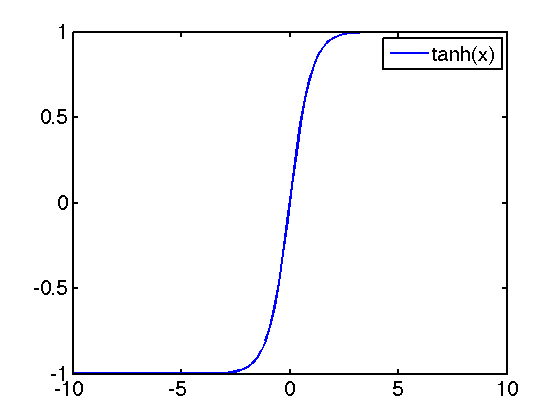
\includegraphics[width=.6\linewidth]{tanh.png}
%\caption{default}
\label{fig:tanh}
\end{center}
\end{figure}
}

\frame[t] {% slide 3
 \frametitle{tanh regression (like logistic regression)}

For pedagogical purpose assume that $\tanh()$ can't be inverted.
\bigskip

Or that we observe targets that are $t_n \in \{-1, +1\}$ (note -- not continuous valued!)
\bigskip

Let's consider a regression(/classification) function 

\[ y(\xbf_n,\wbf) = \tanh(\xbf_n\wbf) \] 

where $\wbf$ is a parameter vector and $\xbf$ is a vector of inputs (potentially features).  For each input $\xbf$ we have an observed output $t_n$ which is either minus one or one. 
\bigskip

We are interested in the general case of how to learn parameters for such models.
}

\frame[t] {% slide 4
 \frametitle{tanh regression (like logistic regression)}

Further, we will use the error that you are familiar with, namely, the squared error.  So, given a matrix of inputs $\Xbf = [ \xbf_1 \cdots \xbf_n]$ and a collection of output labels $\tbf = [t_1 \cdots t_n]$ we consider the following squared error function
 
\[E(\Xbf, \tbf, \wbf) = \frac{1}{2} \sum_n (t_n - y(\xbf_n, \wbf))^2\]

We are interested in minimizing the error of our regressor/classifier.  \\

How do we do this?
}

\frame[t] {% slide 5
 \frametitle{Error minimization}

If we want to minimize 

\[E(\Xbf, \tbf, \wbf) = \frac{1}{2} \sum_n (t_n - y(\xbf_n, \wbf))^2\]

w.r.t. $\wbf$ we should start by deriving gradients and trying to find places where the they disappear.
\bigskip
\begin{figure}[htbp]
\begin{center}
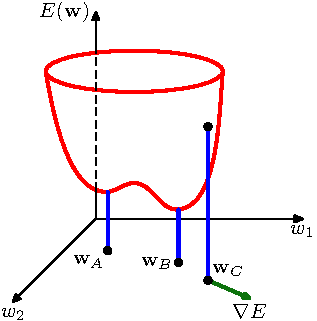
\includegraphics[width=.4\linewidth]{../prmlfigs-pdf-recolored/Figure5_5.pdf}
%\caption{default}
\label{fig:minimization}
\end{center}
\end{figure}
{\tiny Figure taken from PRML, Bishop 2006}
}

\frame[t] {% slide 6
 \frametitle{Error gradient w.r.t.~$\wbf$}

The gradient of 
\begin{eqnarray*}
\nabla_\wbf E(\Xbf, \tbf, \wbf) &=& \frac{1}{2} \sum_n \nabla_\wbf (t_n - y(\xbf_n, \wbf))^2 \\
 &=&-\sum_n(t_n - y(\xbf_n, \wbf)) \nabla_\wbf y(\xbf_n, \wbf)
\end{eqnarray*}

A useful fact to know about $\tanh()$ is that \[\frac{d\tanh(a)}{db} = (1-\tanh(a)^2)\frac{da}{db}\]

which makes it easy to complete the last line of the gradient computation straightforwardly for the choice of $y(\xbf_n,\wbf) = \tanh(\xbf_n\wbf)$, namely

\begin{eqnarray*}
\nabla_\wbf E(\Xbf, \tbf, \wbf) &=& -\sum_n(t_n - y(\xbf_n, \wbf))(1-\tanh(\xbf_n\wbf)^2)\xbf_n
\end{eqnarray*}

}

\frame[t] {% slide 7
 \frametitle{Solving}
It is clear that algebraically solving 
\begin{eqnarray*}
\nabla_\wbf E(\Xbf, \tbf, \wbf) &=& -\sum_n(t_n - y(\xbf_n, \wbf))(1-\tanh(\xbf_n\wbf)^2)\xbf_n \\
&=& \0bf
\end{eqnarray*}
for all the entries of $\wbf$ will be troublesome if not impossible. 
\bigskip

This is OK, however, because we don't always have to get an analytic solution that directly gives us the value of $\wbf$.  We can arrive at it's value numerically.
}

\frame[t] {% slide 8
 \frametitle{Calculus 101}
Even simpler -- consider {\em numerically} minimizing the function 
\begin{figure}[htbp]
\begin{center}
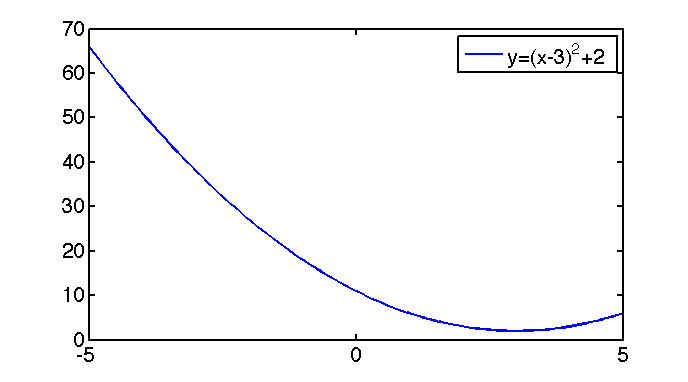
\includegraphics[width=.8\linewidth]{quadratic.png}
%\caption{default}
\label{fig:quadratic}
\end{center}
\end{figure}

How do you do this?
\bigskip

Hint, start at some value $x_0$, say $x_0=-3$ and use the gradient to ``walk'' towards the minimum.

}


\frame[t] {% slide 9
 \frametitle{Calculus 101}
The gradient of $y=(x-3)^2 +2$ (or derivative w.r.t.~$x$) is $\nabla_x y = 2(x-3)$.
\bigskip

Consider the sequence $x_n  = x_{n-1} - \lambda \nabla_{x_{n-1}} y$
\bigskip

It is clear that if $\lambda$ is small enough that this sequence will converge  to $\lim_{n\rightarrow\infty} x_n \rightarrow 3$.
\bigskip

There are several important caveats worth mentioning here

\begin{itemize}
\item If $\lambda$ (called the learning rate) is set too high this sequence might oscillate
\item Worse yet, the sequence might diverge.
\item If the function has multiple minima (and/or saddles) this procedure is {\em not} guaranteed to converge to the minimum value.
\end{itemize}

}

\frame[t] {% slide 10
 \frametitle{Arbitrary error gradients}

This is true for any function that one would like to minimize.  
\bigskip

For instance we are interested in minimizing prediction error $E(\Xbf, \tbf, \wbf)$ in our ``logistic'' regression/classification example where the gradient we computed is

\begin{eqnarray*}
\nabla_\wbf E(\Xbf, \tbf, \wbf) &=& -\sum_n(t_n - y(\xbf_n, \wbf))(1-\tanh(\xbf_n\wbf)^2)\xbf_n
\end{eqnarray*}

So starting at some value of the weights $\wbf_0$ we can construct and follow a sequence of guesses until convergence

\[\wbf_n  =\wbf_{n-1} - \lambda \nabla_{\wbf_{n-1}} E(\Xbf, \tbf, \wbf)\]

}

\frame[t] {% slide 11
 \frametitle{Arbitrary error gradients}
Convergence of a procedure like
\[\wbf_n  =\wbf_{n-1} - \lambda \nabla_{\wbf_{n-1}} E(\Xbf, \tbf, \wbf)\]
can be assessed in multiple ways:
\begin{itemize}
\item The norm of the gradient grows sufficiently small
\item The function value change is sufficiently small from one step to the next.
\item etc.
\end{itemize}

}

\frame[t] {% slide 12
 \frametitle{Gradient Min(Max)imization}

There are several other important points worth mentioning here and avenues for further study

\begin{itemize}
\item If the objective function is {\em convex}, such learning strategies are guaranteed to converge to the global optimum.  Special techniques for convex optimization exist (e.g.~Boyd and Vandenberghe, http://www.stanford.edu/$\sim$boyd/cvxbook/).
\item If the objective function is not convex, multiple restarts of the learning procedure should be performed to ensure reasonable coverage of the parameter space. 
\item Even if the objective is not convex it might be worth the computational cost of restarting multiple times to achieve a good set of parameters.  
\item The ``sum over observations'' nature of the gradient calculation makes online learning feasible.
\item More (much more) sophisticated gradient search algorithms exist, particularly ones that make use of the curvature of the underlying function.
\end{itemize}

}

\frame[t] {% slide 13
 \frametitle{Example - Data for tanh regression/classification}

\begin{figure}[htbp]
\begin{center}
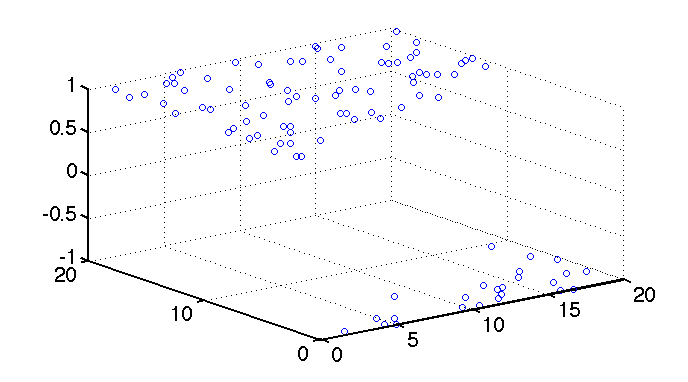
\includegraphics[width=.85\linewidth]{log_reg_data.png}
\caption{Data in $\{+1,-1\}$}
\label{fig:log_reg_data}
\end{center}
\end{figure}

 {\tiny``Generative model'' = 
\begin{quote}
n = 100;\\
x = [rand(n,1) rand(n,1)]*20;\\
y = x*[-2;4] $>$ 2;\\
y = y+ (y==0)*-1;\\
\end{quote}}


}

\frame[t] {% slide 14
 \frametitle{Example - Result from Learning}

\begin{figure}[htbp]
\begin{center}
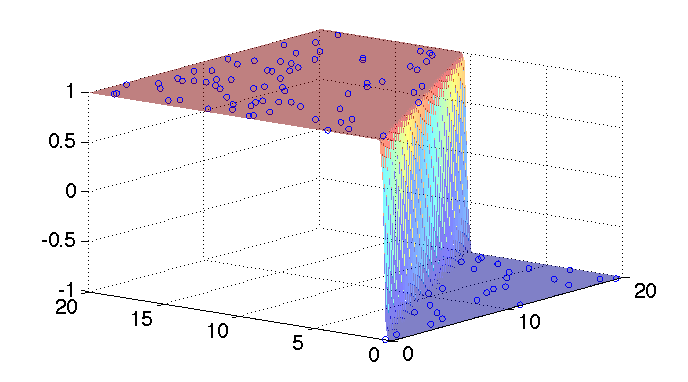
\includegraphics[width=.85\linewidth]{logistic_regression.png}
\caption{Learned regression surface.}
\label{fig:log_reg_data}
\end{center}
\end{figure}

 {\tiny Run logistic\_regression/tanh\_regression.m}


}


\frame[t] {% slide 15
 \frametitle{Two more hints}

\begin{enumerate}
\item Even analytic gradients are not required!
\item (Good) software exists to allow you to minimize whatever function you want to minimize (matlab: fminunc)
\end{enumerate}

For both, note the following.  The definition of a derivative (gradient) is given by

\[\frac{df(x)}{dx} = \lim_{\delta \rightarrow 0} \frac{f(x+\delta ) - f(x)}{\delta }\]

but can be approximated quite well by a fixed size choise of $\delta $, i.e.

\[\frac{df(x)}{dx} \approx  \frac{f(x+.00000001) - f(x)}{.00000001}\]

This means that learning algorithms can be implemented on a computer using given nothing but the objective function to minimize!

}
 \section{Neural Networks}

\frame[t] {% slide 16
 \frametitle{Neural Networks}

It is from this perspective that we will approach neural networks. 
\bigskip

A general two layer feedforward neural network is given by :

\[ y_k(\xbf,\wbf) = \sigma\left(\sum_{j=0}^M w_{kj}^{(2)} h \left(\sum_{i=0}^D w_{ji}^{(1)}x_i \right)\right)\]

\bigskip

Given what we have just covered, if given as set of targets $\tbf = [t_1 \cdots t_n]$ and a set of inputs $\Xbf = [\xbf_1 \cdots \xbf_n]$ one should straightforwardly be able to learn $\wbf$ (the set of all weights $w_{kj}$ and $w_{ji}$ for all combinations $kj$ and $ji$) for any choice of $\sigma()$ and $h()$.
}

\frame[t] {% slide 16
 \frametitle{Neural Networks}

It is from this perspective that we will approach neural networks. 
\bigskip

A general two layer feedforward neural network is given by :

\[ y_k(\xbf,\wbf) = \sigma\left(\sum_{j=0}^M w_{kj}^{(2)} h \left(\sum_{i=0}^D w_{ji}^{(1)}x_i \right)\right)\]

\bigskip

Given what we have just covered, if given as set of targets $\tbf = [t_1 \cdots t_n]$ and a set of inputs $\Xbf = [\xbf_1 \cdots \xbf_n]$ one should straightforwardly be able to learn $\wbf$ (the set of all weights $w_{kj}$ and $w_{ji}$ for all combinations $kj$ and $ji$) for any choice of $\sigma()$ and $h()$.
}

\frame[t] {% slide 16
 \frametitle{Neural Networks}

Neural networks arose from trying to create mathematical simplifications or representations of the kind of processing units used in our brains.
\bigskip

We will not consider their biological feasibility, instead we will focus on a particular class of neural network -- the multi-layer perceptron, which has proven to be of great practical value in both regression and classification settings.
\bigskip
}
\frame[t] {% slide 16
 \frametitle{Neural Networks}
To start -- there should be list of important features and caveats
\begin{enumerate}
\item Neural networks are {\em universal approximators}, meaning that
\begin{quote}a two-layer network with linear outputs can uniformly approximate any continuous function on a compact input domain to arbitrary accuracy provided that the network has a sufficiently large number of hidden units [Bishop, PRML, 2006] \end{quote}
\item {\em but...} How many hidden units?
\item Generally the error surface as a function of the weights is non-convex leading to a difficult and tricky optimization problem.
\item The internal mechanism by which the network represents the regression relationship is not usually examinable or testable in the way that linear regression models are.  i.e.~What's the meaning of a statement like, the 95\% confidence interval for the $i^{th}$ hidden unit weight is $[.2, .4]$?
\end{enumerate}


}

\frame[t] {% slide 17
 \frametitle{Neural network architecture}

\begin{figure}[htbp]
\begin{center}
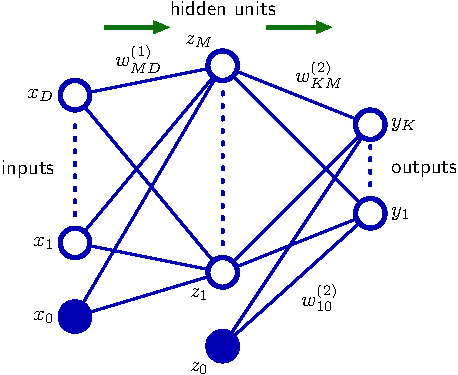
\includegraphics[width=.75\linewidth]{../prmlfigs-pdf-recolored/Figure5_1.pdf}
%\caption{default}
\label{fig:neural_network_arch}
\end{center}
\end{figure}
{\tiny Figure taken from PRML, Bishop 2006}
}


\frame[t] {% slide 18
 \frametitle{Neural Networks}

The specific neural network we will consider is a univariate regression network where there is one output node and the output nonlinearity is set to the identity $\sigma(x) = x$ leaving only the hidden layer nonlinearity $h(a)$ which will will choose to be $h(a) = \tanh(a)$.  So

\[ y_k(\xbf,\wbf) = \sigma\left(\sum_{j=0}^M w_{kj}^{(2)} h \left(\sum_{i=0}^D w_{ji}^{(1)}x_i \right)\right)\]

simplifies to 

\[ y(\xbf,\wbf) = \sum_{j=0}^M w_{kj}^{(2)} h \left(\sum_{i=0}^D w_{ji}^{(1)}x_i \right)\]

Note that the bias nodes $x_0=1$ and $z_0=1$ are included in this notation.  

}

\frame[t] {% slide 19
 \frametitle{Representational Power}
\begin{figure}[htbp]
\begin{center}
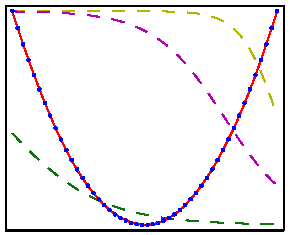
\includegraphics[width=.35\linewidth]{../prmlfigs-pdf-recolored/Figure5_3a.pdf}
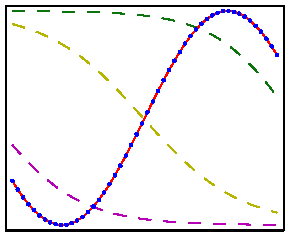
\includegraphics[width=.35\linewidth]{../prmlfigs-pdf-recolored/Figure5_3b.pdf}\\
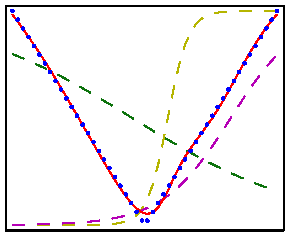
\includegraphics[width=.35\linewidth]{../prmlfigs-pdf-recolored/Figure5_3c.pdf}
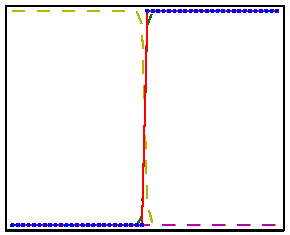
\includegraphics[width=.35\linewidth]{../prmlfigs-pdf-recolored/Figure5_3d.pdf}
%\caption{default}
\label{fig:neural_network_rep_power}
\end{center}
\end{figure}
Four regression functions learned using linear/tanh neural network with three hidden units.  Hidden unit activation shown in the background colors.\\
 
{\tiny Figure taken from PRML, Bishop 2006}
}

\frame[t] {% slide 19
 \frametitle{Neural Network Training}
 
 Given a set of input vectors $\{\xbf_n\}, n=1,\ldots,N$ and a set of target vectors $\{\tbf_n\}$ (taken here to be univariate $\{t_n\}$) we wish to minimize the error function
 
\[ E(\wbf) = \frac{1}{2} \sum_{n=1}^N || y(\xbf_n,\wbf)-t_n||^2\]  
 In this example we will assume that $t\in\mathbb{R}$ and that $t_n$ is Gaussian distributed with mean a function of $\xbf$
 
  \[P(t_n | \xbf,\wbf, \beta) = \mathcal{N}(t_n | y(\xbf_n, \wbf), \beta^{-1})\]

which means that the targets are jointly distributed according to
 
 \[P(\tbf | \Xbf,\wbf, \beta) = \prod_{n=1}^N P(t_n | \xbf_n, \wbf, \beta)\]

}


\frame[t] {% slide 19
 \frametitle{Neural Network Training and Prediction}
 If we take the negative logarithm of the error function
  \[P(\tbf | \Xbf,\wbf, \beta) = \prod_{n=1}^N P(t_n | \xbf_n, \wbf, \beta)\]
we arrive at
\[ \frac{\beta}{2} \sum_{n=1}^N \{ y(\xbf_n,\wbf)-t_n\}^2 - \frac{N}{2} \ln \beta + \frac{N}{2} \ln(2\pi)\]
  which we can minimize by first minimizing w.r.t. to $\wbf$ and then $\beta$.  
  \bigskip
  
  Given a trained value of $\beta_{ML}$ and $\wbf_{ML}$ prediction is straightforward.
  
}

\frame[t] {% slide 19
 \frametitle{Neural Network Training, Gradient Ascent}
We therefore are interested in minimizing (in the case of continuous valued, univariate, neural network regression) 

\[ E(\wbf) = \sum_{n=1}^N \{ y(\xbf_n,\wbf)-t_n\}^2\]

where 

\[ y(\xbf,\wbf) = \sum_{j=0}^M w_{j}^{(2)} h \left(\sum_{i=0}^D w_{ji}^{(1)}x_i \right)\]

which we can perform numerically if we have gradient information

\[ \wbf^{(\tau+1)} = \wbf^{(\tau)} - \eta \nabla E(\wbf^{(\tau)} )\]
  
  where $\eta$ is a learning rate and $ \nabla E(\wbf^{(\tau)}) $ is the gradient of the error function.
}

\frame[t] {% slide 19
 \frametitle{Back Propagation}
While numeric gradient computation can be used to estimate the gradient and thereby adjust the weights of the neural net, doing so is not very efficient.  
\bigskip

A more efficient, if not slightly more confusing method of computing the gradient, is to use {\em backpropagation}.  
\bigskip

Back propagation is a fancy term for a dynamic programming-like way of computing the gradient by running computations backwards on the network.  
}

\frame[t] {% slide 19
 \frametitle{Back Propagation}

To perform back propagation we need to identify several intermediate variables, the first of which is
\[ a_j = \sum_i w_{ji}z_i\]
where $a_j$ is a weighted sum of the inputs to a particular unit (hidden or otherwise).  The activiation $z_j$ of a unit is given by 
\[ z_j = h(a_j)\]
where in our example $h(a) = \tanh(a)$
\bigskip

Here $j$ could be an output.
\bigskip

}

\frame[t] {% slide 19
 \frametitle{Back Propagation}
What we are interested in computing efficiently is $\frac{dE}{dw_{ji}}$ where
\[ E(\wbf) = \sum_{n=1}^N \{ y(\xbf_n,\wbf)-t_n\}^2\]

we will focus on the individual contribution from a single training input/output pair $\frac{dE_n}{dw_{ji}}$ realizing that the final gradient is the sum of all of the individual gradients.  
\bigskip

Note: {\em Stochatistic gradient ascent approximates the gradient using a single (or small group) of points at a time.}

}


\frame[t] {% slide 19
 \frametitle{Back Propagation : Reuse of computation}

Our goal is to reuse computation as much as possible.  We will do this by constructing a back-ward chaining set of partial derivatives that use computation closer to the output nodes in the calculation of the gradients of the error w.r.t. to weights closer to the input nodes.
\bigskip

To start, note that $E_n$ depends on the weights $w_{ji}$ only through the input $a_j$ to unit $j$ (here the unit is again an arbitrary unit).   For this reason we can apply the chain rule to give
\[ \frac{dE_n}{dw_{ji}} = \frac{dE_n}{da_j}\frac{da_j}{dw_{ji}} \]

We will denote $\frac{dE_n}{da_j} = \delta_j$.  The $\delta_j$'s are going to be the quantities we use for dynamic programming.

}

\frame[t] {% slide 19
 \frametitle{Back Propagation : Reuse of computation}
 
 If we remember that 
 
\[ a_j = \sum_i w_{ji}z_i\]

and our new notation  $\frac{dE_n}{da_j} = \delta_j$.  

We can re-write 

\[ \frac{dE_n}{dw_{ji}} = \frac{dE_n}{da_j}\frac{da_j}{dw_{ji}} \]

as

\[ \frac{dE_n}{dw_{ji}} =\delta_j z_i \]

This is almost it!

}

\frame[t] {% slide 19
 \frametitle{Back Propagation : Reuse of computation}
 
For the output layer we have 

\[\frac{dE_n}{da_k} = \frac{d}{da_k}  \frac{1}{2} (a_k - t)^2= y_k  - t_k\]
 
 From this we can compute the gradient with respect to all of the weights leading to the output layer simply using
 \[ \frac{dE_n}{dw_{ki}} =\delta_k z_i \]
 where $i$ ranges over the hidden layer closest to the output layer and $z_i$ are the activations of that layer.
 \bigskip
 
 What remains is to figure out how to use the precomputed $\delta$'s to compute the gradients at all remaining hidden layers back to the input nodes.  For this we need the chain rule from calculus again.

}

\frame[t] {% slide 20
 \frametitle{Back Propagation : Reuse of computation}
 
We want a way of computing $\delta_j$, the ``error'' term for an arbitrary hidden unit as a function of the weights and the error terms already computed closer to the output node(s).   The definition of $\delta_j$ is $\delta_j = \frac{dE_n}{da_j}$
 \bigskip
 
When node $j$ is connected to nodes $k, k=1,\ldots,K$ the following is true: the error is a function of the activations at all $k$ nodes and that the activations at each of these nodes is a function of the activation at node $j$.  That means the following is true (by the chain rule for differentiation)

\[ \frac{dE_n}{da_j} = \sum_k \frac{dE_n}{da_k} \frac{da_k}{da_j} \]
 
 but we have computed $\delta_k = \frac{dE_n}{da_k}$ already for nodes closer to the output already!
}

\frame[t] {% slide 20
 \frametitle{Back Propagation : Reuse of computation}
 
 To summarize, we know 
 
\[ \frac{dE_n}{da_j} = \sum_k \delta_k \frac{da_k}{da_j} \]
 
 We also know $a_k = \sum_j w_{kj}z_j$ and $z_j = h(a_j)$.
 
 This means that 
 \[ \delta_j = \frac{dE_n}{da_j} = \sum_k \delta_kh'(a_j) w_{kj} = h'(a_j)  \sum_k  \delta_k w_{kj} \]

This means that we can compute the $\delta$'s backwards, using only information ``local'' to each unit.
\bigskip

Further we know that $\frac{dE_n}{w_{ji}} = \delta_j z_i$ which is the ``error'' at the output side times the activation on the input side.  Since the activations are computed on the forward pass and the errors are computed on the backwards pass we are done!

}

\frame[t] {% slide 20
 \frametitle{Back Propagation : Full procedure}
\begin{block}{Error Backpropagation}
Repeat for all input/output pairs:
\begin{enumerate}
\item Propagate activations forward through the network for an input $\xbf_n$
\item Compute the $\delta$'s for all the units starting at the output layer and proceeding backwards through the network.
\item Compute the contribution to the gradient for that single input (and sum into global gradient computation).
\end{enumerate}

\end{block}
}


\frame[t] {% slide 20
 \frametitle{Conclusion}
Neural networks are a powerful tool for regression analysis.
\bigskip

Neural networks are not without (significant) downsides.  They lack interpretability, they can be difficult to learn, and the model selection issues that arise in any regression problem don't go away.
\bigskip

Further treatment of neural networks include different activation functions, multivalued outputs, classification, and Bayesian neural networks.
\bigskip

Simple trailing question: what would MAP estimation of a neural network look like (with standard weight decay regularization)?
}


\end{document}
